Seperti yang telah dijelaskan pada \ref{sec:alternatif-solusi}, solusi yang dipilih adalah membuat sistem dengan mengkombinasikan Memcached sebagai \textit{in-memory key-value store} dan menggunakan RocksDB sebagai \textit{persistent database}. Replikasi dan \textit{erasure coding} hanya dilakukan pada data persisten yang disimpan pada \textit{database} tersebut.

\subsection{Kebutuhan Sistem}
\label{subsection:system-requirements}

Dari analisis kebutuhan sistem, diturunkan kebutuhan fungsional dan non-fungsional sistem. Kebutuhan ini kemudian dipetakan pada modul-modul yang akan diimplementasikan dalam sistem eksperimen.

\subsubsection{Kebutuhan Fungsional}
\label{subsection:functional-requirements}

Dalam pengembangannya, sistem eksperimen ini harus memenuhi beberapa kebutuhan fungsional. Kebutuhan fungsional ini diturunkan dari analisis kebutuhan pada bagian \ref{sec:analisis-kebutuhan-sistem}. Kebutuhan fungsional sistem adalah sebagai berikut:

\begin{table}[ht]
\centering
\caption{Kebutuhan Fungsional}
\resizebox{\textwidth}{!}{
    \begin{tabular}{|l|p{12cm}|}
    \hline
    \rowcolor{black!10} ID & Deskripsi Kebutuhan \\ \hline
    F-1 & Sistem harus dapat melakukan operasi \textit{read} dan \text{write} pada sebuah \textit{key-value store database} \\ \hline
    F-2 & Sistem harus dapat menyimpan data secara \textit{persistent} \\ \hline
    F-3 & Sistem harus dapat mencatat waktu transaksi dari \textit{request} masuk hingga operasi selesai \\ \hline
    F-4 & Sistem harus dapat meng-\textit{encode} data menggunakan \textit{erasure coding} \\ \hline
    F-5 & Sistem harus dapat merekonstruksi data dari data yang disimpan menggunakan \textit{erasure coding} \\ \hline
    F-6 & Sistem harus dapat mendistribusikan data atau sebagian data ke \textit{node} lain untuk keperluan ketahanan data \\ \hline
    F-7 & Sistem harus dapat dikonfigurasi untuk menggunakan replikasi ataupun \textit{erasure coding} tanpa mengganti konfigurasi lainnya \\ \hline
    F-8 & Sistem harus dapat dikonfigurasi untuk mencapai tingkat ketahanan tertentu tanpa mengganti konfigurasi lainnya \\ \hline
    F-9 & Sistem harus dapat mensimulasikan \textit{request} dengan ukuran data yang bervariasi \\ \hline
    F-10 & Sistem harus dapat menjalankan \textit{request} secara berulang kali dan bervariasi secara otomatis untuk pengumpulan data \\ \hline
    F-11 & Sistem harus dapat melakukan \textit{logging} dari \textit{request} dan operasi untuk kebutuhan analisis \\ \hline
    \end{tabular}
}
\end{table}

\subsubsection{Kebutuhan Non-fungsional}
\label{subsection:non-functional-requirements}

Dalam pengembangannya, sistem eksperimen ini harus memenuhi beberapa kebutuhan non-fungsional. Kebutuhan fungsional ini diturunkan dari bagian \ref{sec:latar-belakang} dan analisis kebutuhan pada bagian \ref{sec:analisis-kebutuhan-sistem}. Kebutuhan non-fungsional sistem adalah sebagai berikut:

\begin{table}[h]
\centering
\caption{Kebutuhan Non-Fungsional}
\resizebox{\textwidth}{!}{
    \begin{tabular}{|l|p{12cm}|}
    \hline
    \rowcolor{black!10} ID & Deskripsi Kebutuhan \\ \hline
    NF-1 & Sistem harus menyediakan \textit{consistency} yang tinggi dengan \textit{request} ke \textit{node} manapun harus menghasilkan hasil yang sama \\ \hline
    NF-2 & Sistem harus memiliki \textit{availability} yang tinggi dengan harus dapat tetap tersedia walaupun beberapa \textit{node} ada dalam kondisi gagal \\ \hline
    NF-3 & Sistem harus menggunakan penyimpanan minimal untuk skalabilitas dan efisensi biaya \\ \hline
    NF-4 & Sistem harus menyediakan \textit{response time} rendah untuk operasi \textit{read} dan \textit{write} \\ \hline
    \end{tabular}
}
\end{table}

\subsection{Modul}
\label{subsection:modules}

Kebutuhan fungsional dan non-fungsional tersebut dipetakan pada modul-modul yang diimplementasikan dalam sistem eksperimen. Setiap modul dirancang untuk memenuhi tujuan spesifik sesuai dengan kebutuhan sistem.

\subsubsection{Database Node}
\label{subsubsection:database-node}

\textit{Database Node} merupakan modul utama yang berperan sebagai \textit{key-value store} pada eksperimen ini. Berdasarkan keputusan yang diambil pada bagian \ref{subsection:modules}, modul ini akan dibuat modular dengan komponen-komponen terpisah. Memcached akan digunakan sebagai \textit{in-memory key-value store} dan RocksDB sebagai \textit{persistent database}. Untuk menggabungkan kedua komponen tersebut, akan dibuat komponen tambahan yang berperan sebagai \textit{controller}.

Komponen \textit{controller} akan berperan untuk mengambil data dari memori jika tersedia dan dari \textit{database} jika data tidak ditemukan di memori untuk operasi \textit{read}. Sementara itu, pada operasi \textit{write}, \textit{controller} akan berperan untuk menyebarkan data yang diproses menggunakan \textit{storage module} ke \textit{database node} lainnya. \textit{Controller} juga akan berperan untuk mengelola konsistensi antar-node menggunakan algoritma konsensus. Penjelasan mengenai peran \textit{database node} pada arsitektur sistem keseluruhan dapat dilihat pada bagian \ref{subsection:system-architecture}.

Merujuk analisis kebutuhan sistem pada bagian \ref{sec:analisis-kebutuhan-sistem}, modul \textit{database node} memenuhi kebutuhan 1 dan 2, yaitu:

\begin{enumerate}
    \item Sistem harus dapat mensimulasikan kondisi \textit{database} terdistribusi yang menggunakan replikasi ataupun \textit{erasure coding}.
    \item Sistem harus dapat menyimpan data secara \textit{persistent} untuk mensimulasikan kegagalan dan pemulihan.
\end{enumerate}

Sedangkan merujuk kebutuhan fungsional dan non-fungsional pada bagian \ref{subsection:system-requirements}, modul ini harus memenuhi kebutuhan fungsional F-1, F-2, F-6, F-7, F-8, dan F-11 serta non-fungsional NF-1, NF-2, NF-3, dan NF-4.

\subsubsection{Storage Module}
\label{subsubsection:storage-module}

Modul ini berfungsi untuk mengatur mekanisme \textit{database node} dalam meningkatkan ketahanan data. Salah satu peran yang dilakukan adalah \text{encode/decode} untuk \textit{erasure coding} data yang diterima dan membaginya ke dalam beberapa bagian \textit{shard} yang kemudian akan dikembalikan pada komponen \textit{controller} pada \textit{database node} untuk didistribusikan. Selain itu, modul ini juga akan menghadirkan pilihan untuk menggunakan replikasi data. Pengkhususan modul ini dari modul-modul lainnya dilakukan untuk mengisolasi perbedaan antara replikasi dan \textit{erasure coding} tanpa mengubah variabel lainnya.

Merujuk pada bagian \ref{sec:analisis-kebutuhan-sistem}, \textit{Storage Module} memenuhi kebutuhan 1, yaitu:

\begin{enumerate}
    \item Sistem harus dapat mensimulasikan kondisi \textit{database} terdistribusi yang menggunakan replikasi ataupun \textit{erasure coding}.
\end{enumerate}

Sedangkan merujuk kebutuhan fungsional dan non-fungsional pada bagian \ref{subsection:system-requirements}, modul ini harus memenuhi kebutuhan fungsional F-4, F-5, dan F-11 serta non-fungsional NF-1, NF-3, dan NF-4.

\subsubsection{Data Collection Module}
\label{subsubsection:data-collection-module}

Modul ini merupakan modul yang berperan untuk melakukan \textit{request} dan melakukan transaksi pada sistem. Hal utama yang akan dilakukan oleh modul ini adalah pengumpulan data dari eksperimen. Oleh karena itu, modul ini akan memiliki fitur yang dapat memvariasikan ukuran data, transaksi, dan \textit{timer} untuk mengukur \textit{response time} dari operasi. Selain itu, modul ini juga perlu dilengkapi dengan otomasi agar dapat menjalankan eksperimen berulang kali untuk mendapatkan data persentil dari eksperimen.

Merujuk pada bagian \ref{sec:analisis-kebutuhan-sistem}, \textit{Data Collection Module} memenuhi kebutuhan 3 dan 4, yaitu:

\begin{enumerate}
    \setcounter{enumi}{2}
    \item Sistem harus dapat memvariasikan ukuran data, tingkat ketahanan, kecepatan jaringan, dan kemampuan komputasi.
    \item Sistem harus dapat menjalankan eksperimen berulang kali untuk mendapatkan data persentil dari eksperimen.
\end{enumerate}

Sedangkan merujuk kebutuhan fungsional dan non-fungsional pada bagian \ref{subsection:system-requirements}, modul ini harus memenuhi kebutuhan fungsional F-3, F-9, F-10, dan F-11

\subsubsection{Modul Lainnya}
\label{subsubsection:other-modules}

Selain ketiga modul yang sudah dijelaskan, akan terdapat beberapa modul minor yang diperlukan untuk meningkatkan kinerja sistem dan mempermudah keberjalanan eksperimen. Contoh modul-modul tersebut antara lain adalah \textit{load balancer}, \textit{logger}, dan \textit{startup-script}. \textit{Load balancer} berfungsi untuk mendistribusikan \textit{request} dari \textit{client} ke \textit{database node} yang tersedia. Modul \textit{logger} berfungsi untuk mencatat kinerja sistem serta memudahkan analisis hasil eksperimen. Sedangkan modul \textit{startup-script} akan membantu pembangunan sistem \textit{key-value store database} secara keseluruhan untuk mengatur konfigurasi ketahanan sistem. Modul-modul ini tidak memiliki peran yang krusial dalam sistem, namun membantu dalam mempermudah pengembangan dan analisis. Dinamika eksperimen tidak menutup kemungkinan adanya modul tambahan yang diperlukan. Beberapa kebutuhan pada poin 4 bagian \ref{sec:analisis-kebutuhan-sistem} akan diimplementasikan melalui \textit{platform} tempat eksperimen dilakukan.

\subsection{Arsitektur Sistem}
\label{subsection:system-architecture}

\begin{figure}[ht]
    \centering
    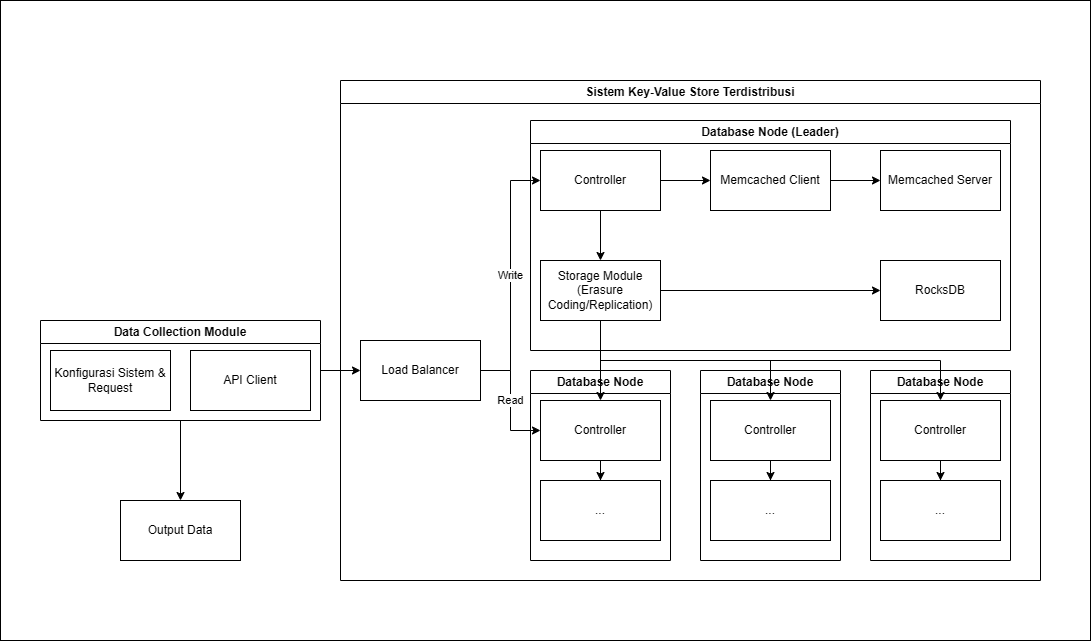
\includegraphics[width=0.95\textwidth]{resources/chapter-3/general-architecture.png}
    \caption{Gambaran Umum Arsitektur Sistem Eksperimen}
    \label{fig:general-architecture}
\end{figure}

Arsitektur dari sistem mengasumsikan kebutuhan untuk konsistensi yang tinggi. Untuk mencapai konsistensi tersebut, operasi \textit{write} dilakukan secara \textit{synchronous} dengan distribusi replikasi dan \textit{erasure coding} dianggap selesai ketika nilai ketahanan yang diinginkan sudah tercapai. Sistem terdistribusi akan mengadopsi pola \textit{leader-follower} untuk memudahkan sinkronisasi data. Pemilihan \textit{leader} dan pemastian transaksi akan dilakukan menggunakan algoritma konsensus \textit{paxos} yang disesuaikan dengan kebutuhan. Diagram gambaran umum arsitektur sistem dapat dilihat pada gambar \ref{fig:general-architecture}.

Operasi akan disalurkan melalui sebuah \textit{load-balancer} sebelum mencapai \textit{database node}. Operasi \textit{write} akan secara ekslusif disalurkan pada \textit{leader}. Kemudian untuk ketahanan, data akan didistribusikan pada \textit{follower} sesuai dengan konfigurasi modul \textit{redundancy}. Sementara itu, operasi \textit{read} dapat dilakukan pada \textit{database node} manapun. Pada sistem \textit{erasure coding}, jika pada \textit{node} tersebut tidak terdapat nilai data yang dicari, maka \textit{node} akan melakukan \textit{request} ke semua node lainnya untuk melakukan rekonstruksi data.

\subsection{Alur Transaksi}
\label{subsection:system-flow}

Alur untuk transaksi \textit{read} dapat dilihat pada gambar \ref{fig:flow-read-mermaidjs} dengan \textit{request} masuk ke \textit{load balancer} kemudian disalurkan ke \textit{database node} yang tersedia. \textit{Database node} akan melakukan operasi \textit{read} pada \textit{key-value store} dan mengembalikan hasil operasi ke \textit{load balancer} untuk dikirimkan ke \textit{client} jika tersedia. Jika tidak, maka \textit{database node} akan melakukan rekonstruksi data dari \textit{erasure-coded persistent data} yang tersebar pada \textit{node-node} lainnya. Pada replikasi, data akan diambil dari \textit{node} lain yang memiliki data yang sama.

\begin{figure}[!ht]
    \centering
    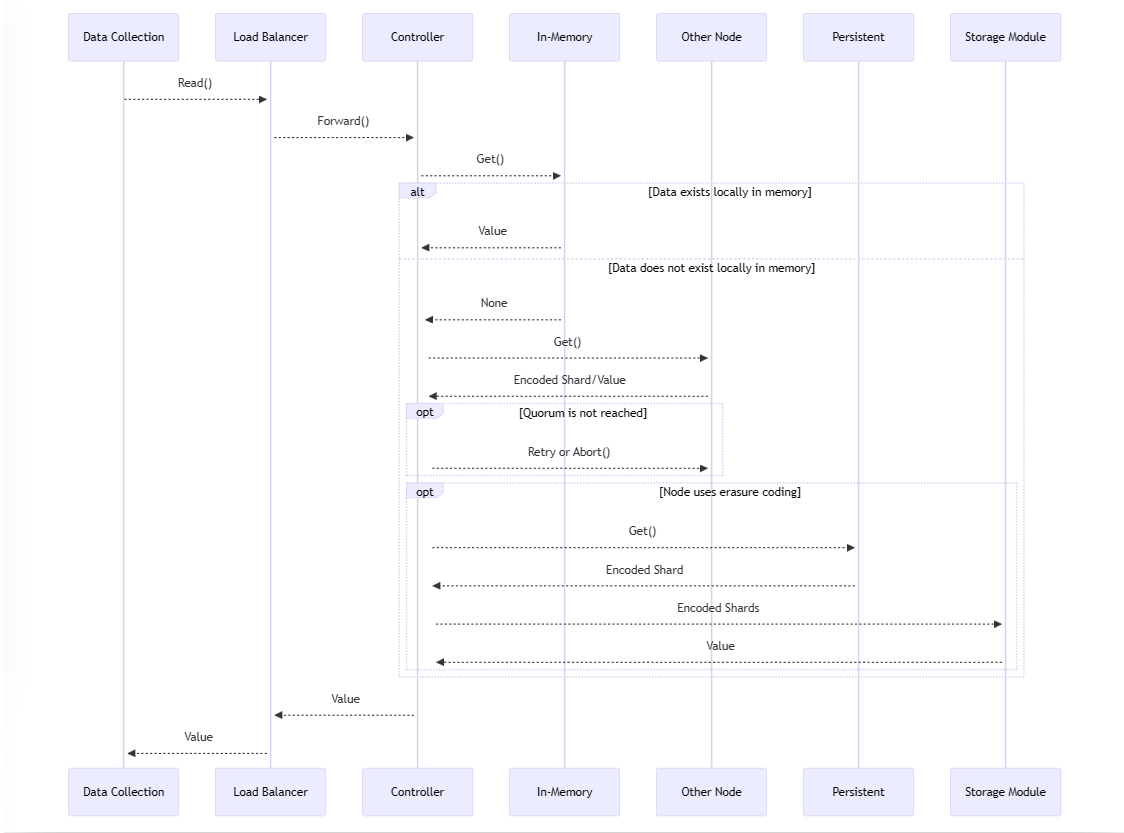
\includegraphics[width=0.95\textwidth]{resources/chapter-3/flow-read-mermaidjs.png}
    \caption{Flow operasi \textit{read} dalam rancangan implementasi}
    \label{fig:flow-read-mermaidjs}
\end{figure}

Alur untuk transaksi \textit{read} dapat dilihat pada gambar \ref{fig:flow-write-mermaidjs} dengan \textit{request} masuk ke \textit{load balancer} kemudian disalurkan ke \textit{database node} yang merupakan leader. Leader kemudian akan melakukan operasi \textit{erasure coding} lalu menyebarkan \textit{shard} ke \textit{follower} yang tersedia. Setelah semua \textit{follower} menerima \textit{shard}, maka operasi \textit{write} dianggap selesai. Operasi \textit{write} pada replikasi juga akan menunggu semua \textit{follower} menerima data sebelum dianggap selesai. 

\begin{figure}[!ht]
    \centering
    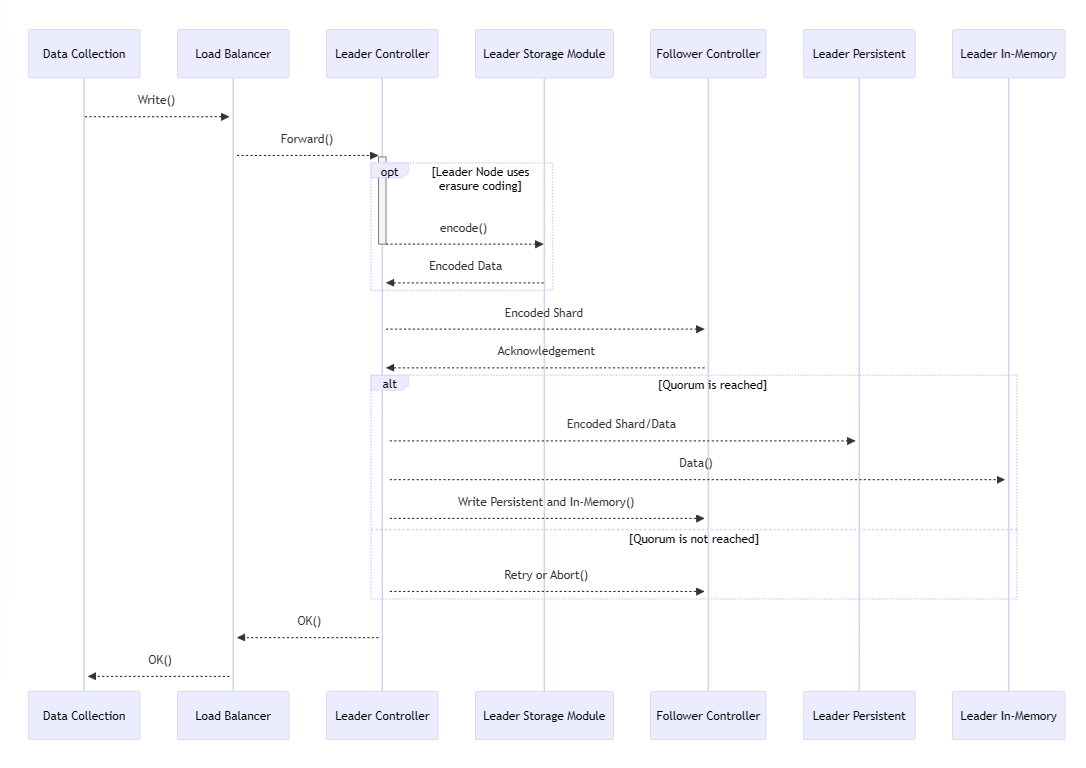
\includegraphics[width=0.95\textwidth]{resources/chapter-3/flow-write-mermaidjs.png}
    \caption{Flow operasi \textit{write} dalam rancangan implementasi}
    \label{fig:flow-write-mermaidjs}
\end{figure}
